\documentclass[tikz, border=1cm]{standalone}

\usepackage{tikz}
\usetikzlibrary{calc}

\begin{document}
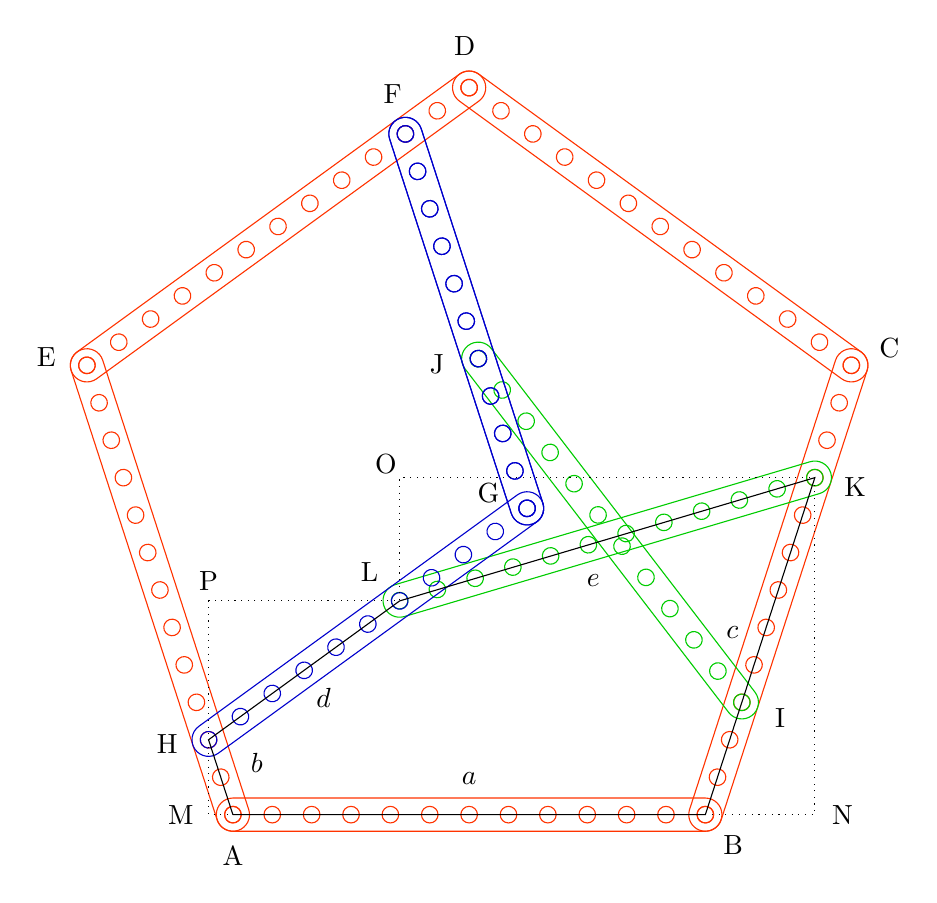
\begin{tikzpicture}

\newcommand{\rod}[4][000000] % [color][n][sep][prop]
{
 \definecolor{main}{HTML}{#1}
 \draw[main] (0,{{2*#4}})
   -- ++({#2*#3},0) arc(+90:-90:{2*#4})
   -- ++({-#2*#3},0) arc(270:90:{2*#4});
 \foreach \x in {0,1,...,#2}
  \draw[main] (\x*#3,0) circle (#4);
}

\def\s {12} \def\f {0.5} \def\p {3pt}
\def\red {FF3300} \def\blue {0000cc} \def\green {00cc00}
\begin{scope}
 \rod[\red]{\s}{\f}{\p} \path (0,0) ++(270:5*\p) node{A};
 \begin{scope}[shift={(\s*\f,0)},rotate=72]
  \rod[\red]{\s}{\f}{\p} \path (0,0) ++(240:5*\p) node{B};
  
  \begin{scope}[shift={(3*\f,0)},rotate=90-34.5]
   \rod[\green]{11}{\f}{\p}
   \path (0,0) ++(210:5*\p) node{I};
   \path (11*\f,0) ++(60:5*\p) node{J};
  \end{scope}
  \begin{scope}[shift={(9*\f,0)},rotate=90+34.5]
   \rod[\green]{11}{\f}{\p}
   \path (0,0) ++(150:5*\p) node{K};
   \path (11*\f,0) ++(-60:5*\p) node{L};
  \end{scope}
  
  
  \begin{scope}[shift={(\s*\f,0)},rotate=72]
   \rod[\red]{\s}{\f}{\p} \path (0,0) ++(240:5*\p) node{C};
   \begin{scope}[shift={(\s*\f,0)},rotate=72]
    \rod[\red]{\s}{\f}{\p} \path (0,0) ++(240:5*\p) node{D};
	
	\begin{scope}[shift={(2*\f,0)},rotate=72]
	 \rod[\blue]{10}{\f}{\p} \path (0,0) ++(180:5*\p) node{F};
	 \rod[\blue]{10}{\f}{\p} \path (10*\f,0) ++(230:5*\p) node{G};
	\end{scope}

    \begin{scope}[shift={(\s*\f,0)},rotate=72]
     \rod[\red]{\s}{\f}{\p} \path (0,0) ++(240:5*\p) node{E};

	 \begin{scope}[shift={(10*\f,0)},rotate=72+36]
	  \rod[\blue]{10}{\f}{\p} \path (0,0) ++(150:5*\p) node{H};
	 \end{scope}


    \end{scope}
   \end{scope}
  \end{scope}
 \end{scope}

\end{scope}

\def\a{12*\f} \def\b{2*\f} \def\c{9*\f} \def\d{6*\f} \def\e{11*\f}

\pgfmathsetmacro{\cosA}{cos(72)}
\pgfmathsetmacro{\sinA}{sin(72)}
\pgfmathsetmacro{\cosB}{cos(36)}
\pgfmathsetmacro{\sinB}{sin(36)}

\coordinate (M) at (-\b*\cosA,0);
\coordinate (A) at (0,0);
\coordinate (B) at (\a,0);
\coordinate (N) at (\a+\c*\cosA,0);
\coordinate (K) at (\a+\c*\cosA,\c*\sinA);
\coordinate (O) at (-\b*\cosA+\d*\cosB,\c*\sinA);
\coordinate (L) at (-\b*\cosA+\d*\cosB,\b*\sinA+\d*\sinB);
\coordinate (P) at (-\b*\cosA,\b*\sinA+\d*\sinB);
\coordinate (H) at (-\b*\cosA,\b*\sinA);

\draw[dotted] (B) 
-- (N) node[shift={(1em,0)}]{N}
-- (K)
-- (O) node[shift={(-0.5em,0.5em)}]{O}
-- (L)
-- (P) node[shift={(0,0.7em)}]{P}
-- (M) node[shift={(-1em,0)}]{M}
-- (A);
 
\draw[] (A)
-- (B) node [midway,yshift=1.3em]{$a$}
-- (K) node [midway,shift={(-1em,.5em)}]{$c$}
-- (L) node [midway,shift={(-.5em,-1.5em)}]{$e$}
-- (H) node [midway,shift={(0.7em,-1em)}]{$d$}
-- (A) node [midway,shift={(1.3em,.5em)}]{$b$};

\end{tikzpicture}
\end{document}
